\section{Model 1: SOC Continuous-Time Dynamics}
\label{sec:model1}

This section develops a continuous-time mathematical model for the battery State of Charge as a function of time, incorporating electrochemical, thermal, and usage-dependent factors. Our approach follows the equivalent circuit modeling framework established by Plett \cite{Plett2015} and validated extensively for Li-ion batteries \cite{Hu2012, Chen2006}.

\subsection{SOC Dynamics: Coulomb Counting}
\label{subsec:soc_dynamics}

The fundamental principle underlying SOC estimation is \textbf{Coulomb counting}, which tracks the cumulative charge flow into or out of the battery \cite{Plett2004}.

\begin{definition}[State of Charge]
SOC is defined as the ratio of remaining charge to total usable capacity:
\begin{equation}
    \SOC(t) = \frac{Q_{\text{remaining}}(t)}{Q_{\text{usable}}}
\end{equation}
\end{definition}

The rate of change of SOC follows directly from the definition:

\begin{equation}
    \boxed{\frac{d\SOC}{dt} = -\frac{I(t)}{\Qnom \cdot \SOH \cdot 3600}}
    \label{eq:soc_dynamics}
\end{equation}

where:
\begin{itemize}
    \item $I(t)$ [A] is the discharge current (positive for discharge)
    \item $\Qnom$ [Ah] is the nominal battery capacity
    \item $\SOH \in [0,1]$ is the State of Health (fraction of original capacity)
    \item The factor 3600 converts Ah to As (Coulombs)
\end{itemize}

\textbf{Physical interpretation:} Equation~\eqref{eq:soc_dynamics} states that SOC decreases proportionally to the current drawn from the battery, scaled by the effective capacity $\Qnom \cdot \SOH$.

\subsection{Second-Order Equivalent Circuit Model (2-RC ECM)}
\label{subsec:ecm}

To capture the dynamic voltage response of the battery, we employ a second-order Equivalent Circuit Model consisting of:

\begin{itemize}
    \item \textbf{OCV source} $\OCV(\SOC, T)$: Represents the thermodynamic equilibrium voltage
    \item \textbf{Ohmic resistance} $R_0$: Instantaneous voltage drop under load
    \item \textbf{Two RC pairs} $(R_1, C_1)$ and $(R_2, C_2)$: Model polarization dynamics at different time scales
\end{itemize}

\begin{figure}[H]
    \centering
    \begin{tikzpicture}[
        component/.style={draw, minimum width=0.8cm, minimum height=0.5cm},
        arrow/.style={->, thick}
    ]
        % OCV source
        \draw (0,0) -- (0,2);
        \node at (0,1) [left] {$V_{\text{OC}}$};
        \draw (0,0) circle (0.15) node [below=0.2cm] {$-$};
        \draw (0,2) circle (0.15) node [above=0.2cm] {$+$};
        
        % R0
        \draw (0.15,2) -- (1,2);
        \draw (1,1.7) rectangle (2,2.3);
        \node at (1.5,2) {$R_0$};
        \draw (2,2) -- (2.5,2);
        
        % RC1
        \draw (2.5,2) -- (2.5,2.5) -- (3,2.5);
        \draw (3,2.2) rectangle (4,2.8);
        \node at (3.5,2.5) {$R_1$};
        \draw (4,2.5) -- (4.5,2.5) -- (4.5,2);
        
        \draw (2.5,2) -- (2.5,1.5) -- (3,1.5);
        \draw (3.2,1.3) -- (3.2,1.7);
        \draw (3.4,1.2) -- (3.4,1.8);
        \node at (3.8,1.5) {$C_1$};
        \draw (3.6,1.5) -- (4.5,1.5) -- (4.5,2);
        
        % RC2
        \draw (4.5,2) -- (5,2);
        \draw (5,2) -- (5,2.5) -- (5.5,2.5);
        \draw (5.5,2.2) rectangle (6.5,2.8);
        \node at (6,2.5) {$R_2$};
        \draw (6.5,2.5) -- (7,2.5) -- (7,2);
        
        \draw (5,2) -- (5,1.5) -- (5.5,1.5);
        \draw (5.7,1.3) -- (5.7,1.7);
        \draw (5.9,1.2) -- (5.9,1.8);
        \node at (6.3,1.5) {$C_2$};
        \draw (6.1,1.5) -- (7,1.5) -- (7,2);
        
        % Output
        \draw (7,2) -- (8,2);
        \draw (0.15,0) -- (8,0);
        \node at (8,2) [right] {$V(t)$};
        \node at (8,0) [right] {GND};
        
        % Current arrow
        \draw[arrow] (7.5,2.5) -- (7.5,2.1);
        \node at (7.5,2.7) {$I(t)$};
        
    \end{tikzpicture}
    \caption{Second-order Equivalent Circuit Model (2-RC ECM) for Li-ion battery.}
    \label{fig:ecm}
\end{figure}

To provide intuition for how internal battery states translate to measurable terminal voltage, Figure~\ref{fig:ecm_concentric} presents a novel \textbf{concentric layer visualization}. This representation emphasizes that SOC (the core state) can only be inferred indirectly through the ``electrical layers'' of polarization dynamics.

\begin{figure}[H]
    \centering
    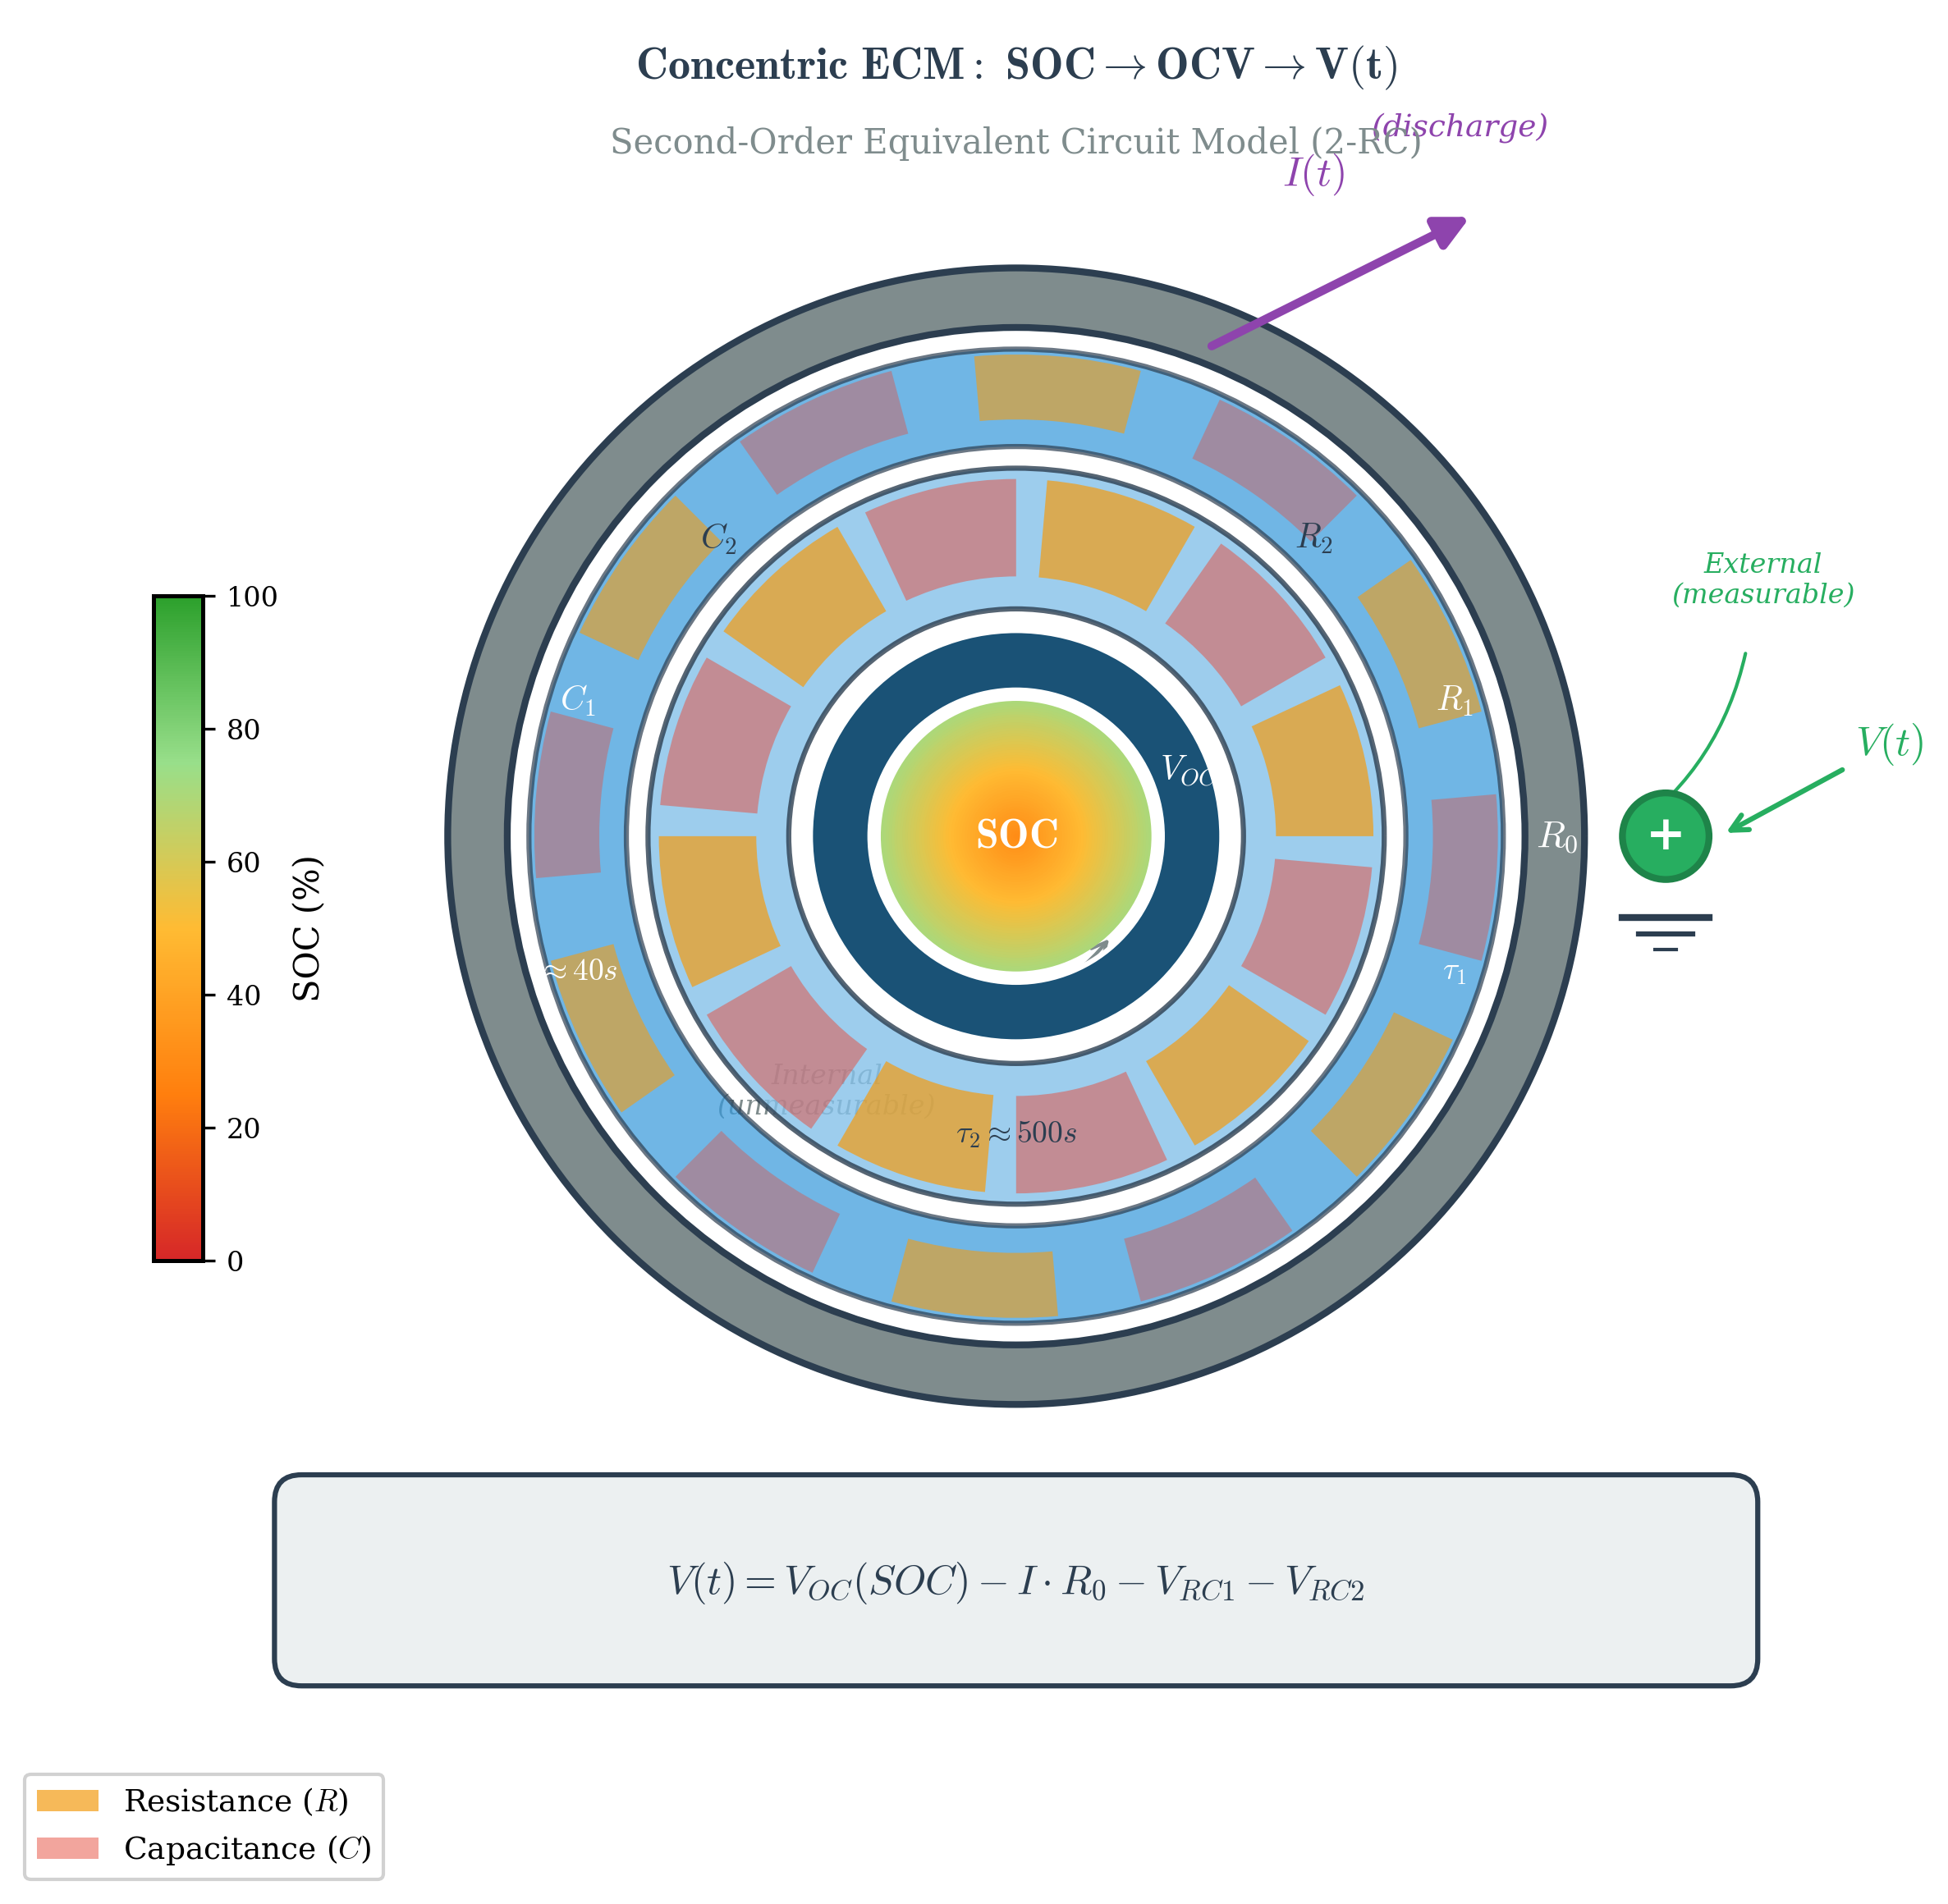
\includegraphics[width=0.85\textwidth]{figures/ecm_concentric.png}
    \caption{Concentric layer representation of the 2-RC ECM. The internal SOC (center) is obscured by successive electrochemical layers: OCV source, slow polarization ($\tau_2 \approx 500$s), fast polarization ($\tau_1 \approx 40$s), and ohmic resistance. Only the terminal voltage $V(t)$ is directly measurable.}
    \label{fig:ecm_concentric}
\end{figure}

The RC branch voltages follow first-order dynamics:

\begin{align}
    \frac{dV_{RC1}}{dt} &= -\frac{V_{RC1}}{\tau_1(T)} + \frac{I(t)}{C_1} \label{eq:vrc1} \\
    \frac{dV_{RC2}}{dt} &= -\frac{V_{RC2}}{\tau_2(T)} + \frac{I(t)}{C_2} \label{eq:vrc2}
\end{align}

where $\tau_i = R_i C_i$ are the time constants (temperature-dependent).

\subsubsection{RC Dynamics Visualization}

To illustrate how the RC polarization dynamics affect voltage response, Figure~\ref{fig:rc_dynamics} shows simulated responses to current pulses and the corresponding SOC evolution.

\begin{figure}[H]
    \centering
    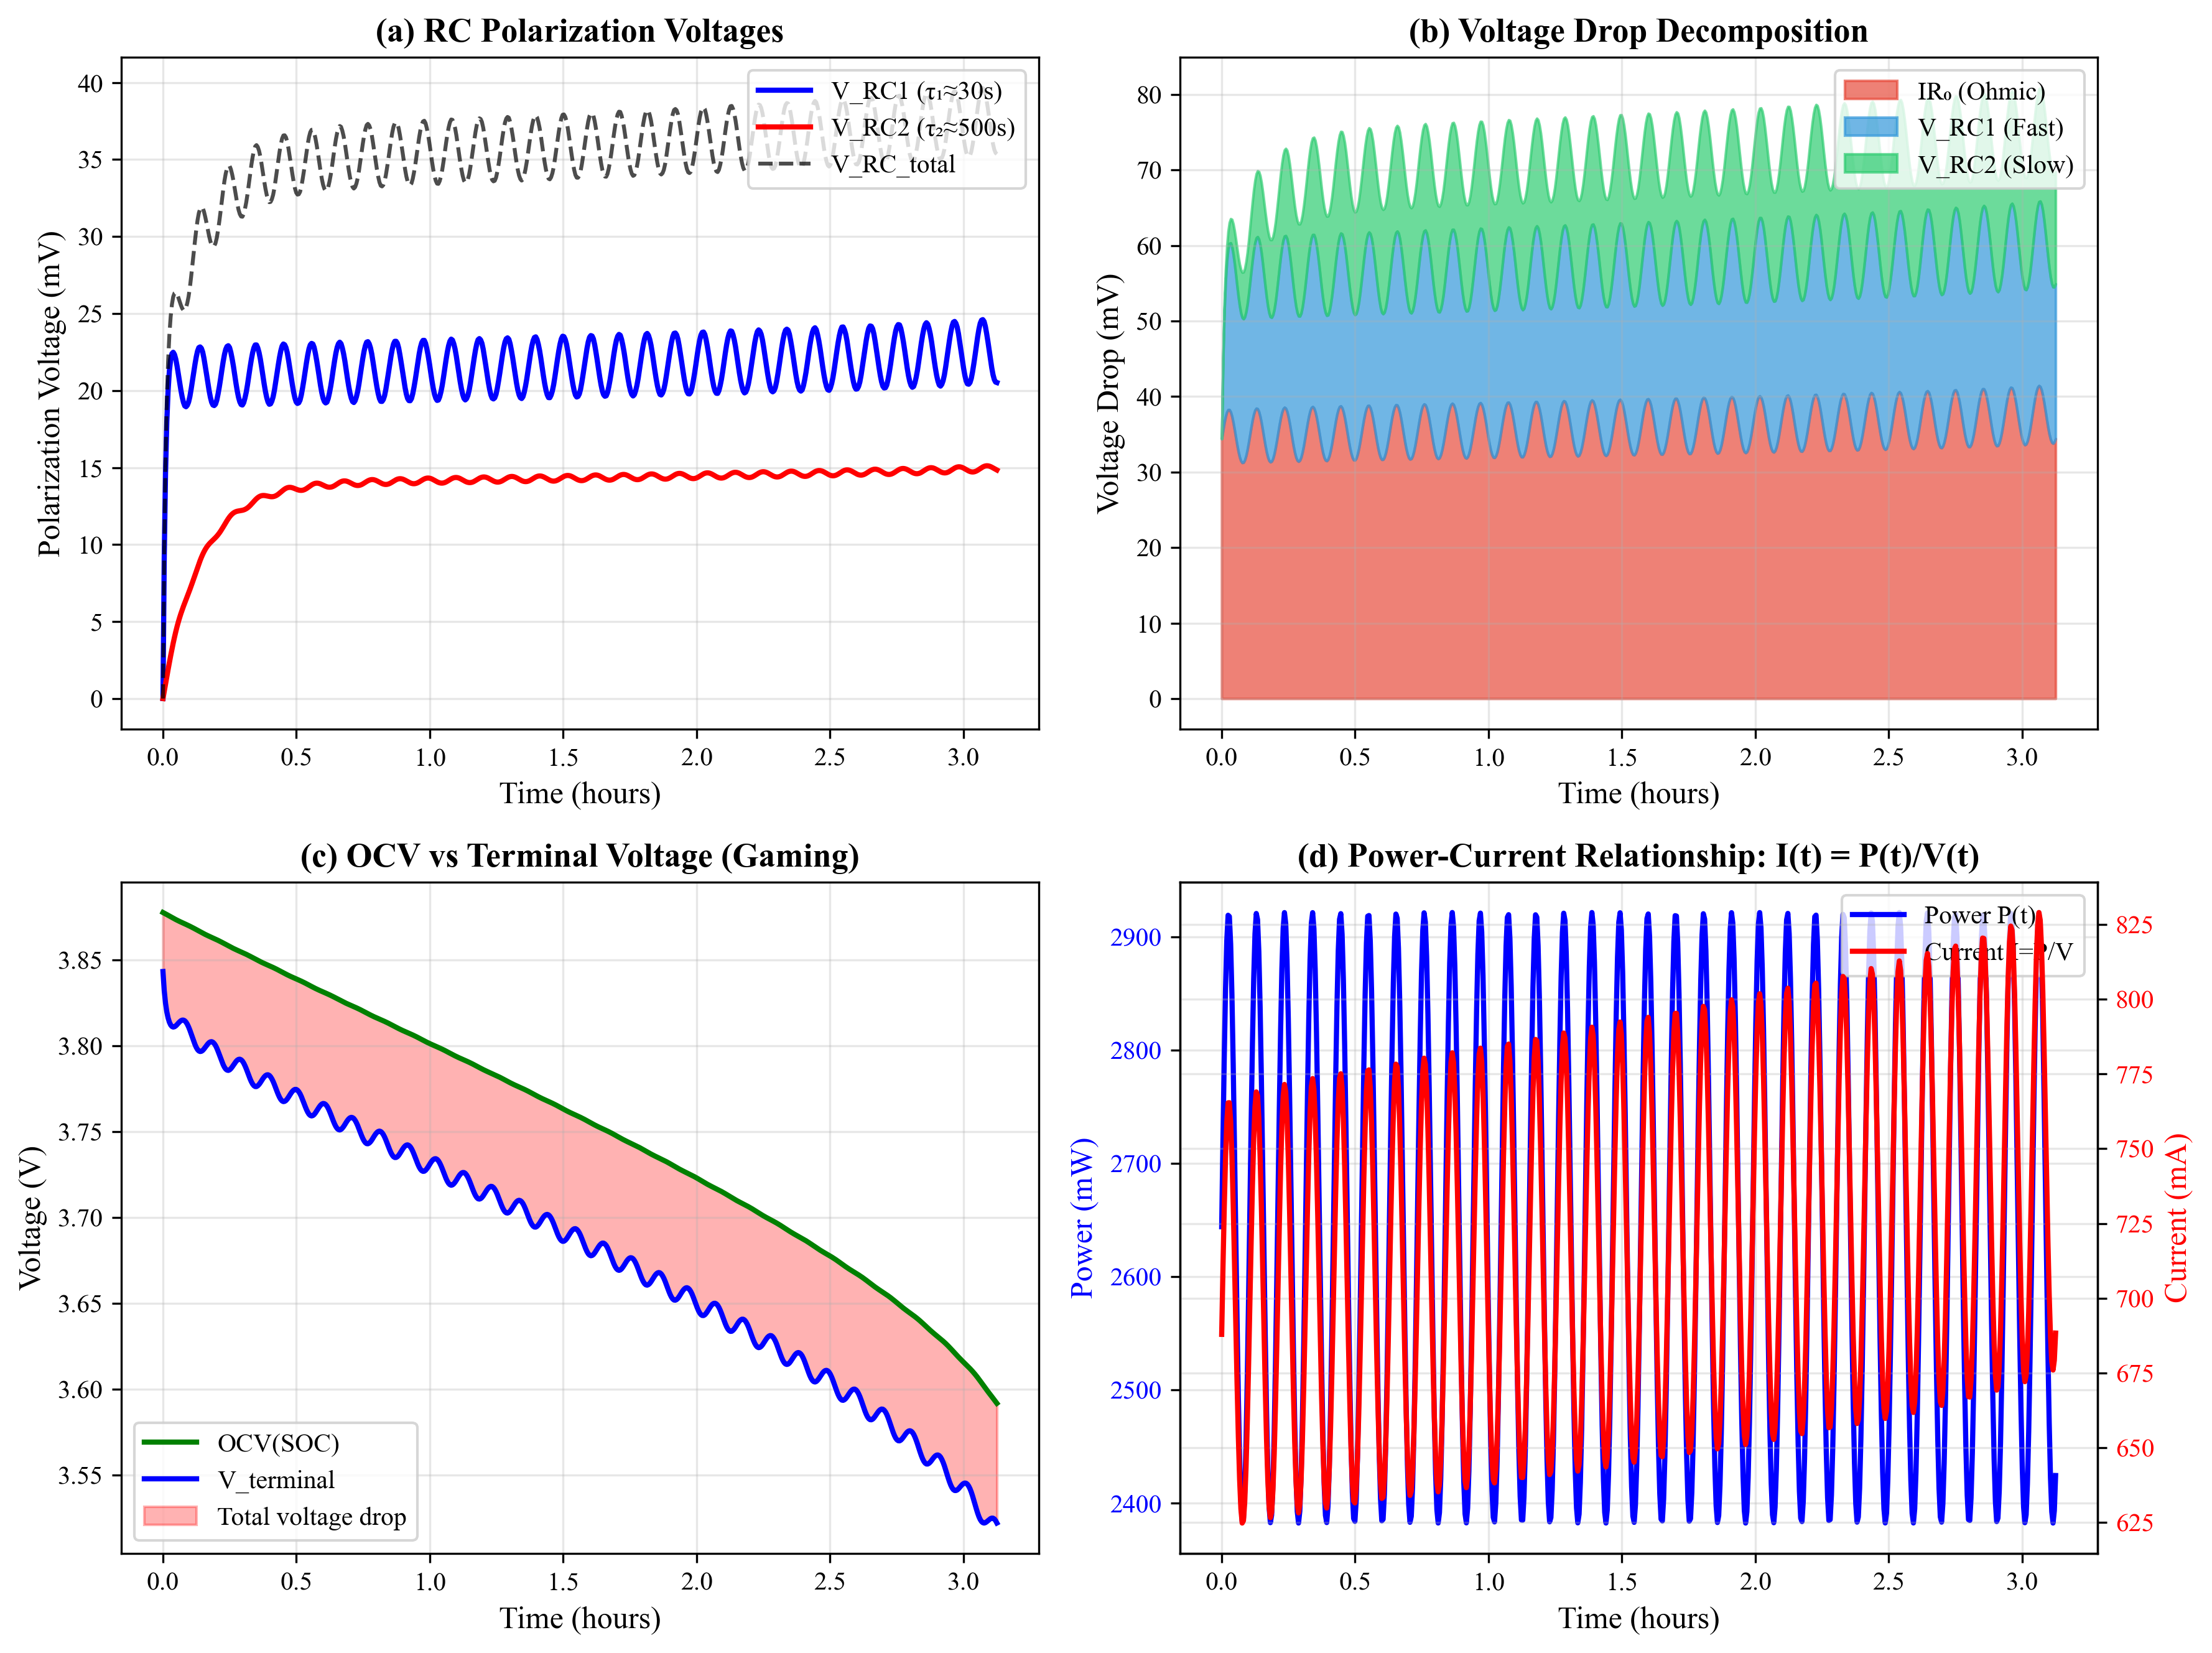
\includegraphics[width=\textwidth]{figures/rc_dynamics.png}
    \caption{RC circuit dynamics under realistic loading. \textbf{(a)} Current profile with discharge pulses; \textbf{(b)} Fast and slow RC polarization voltages; \textbf{(c)} Terminal voltage response showing instantaneous drop (R$_0$) and gradual decay (RC); \textbf{(d)} Corresponding SOC evolution.}
    \label{fig:rc_dynamics}
\end{figure}

\subsection{Open-Circuit Voltage Model}
\label{subsec:ocv}

The Open-Circuit Voltage (OCV) represents the thermodynamic equilibrium potential of the battery and is a critical component for accurate SOC estimation. We develop the OCV model through a progression from theoretical electrochemistry to practical implementation.

\subsubsection{From Nernst Equation to Shepherd Model}

The theoretical foundation begins with the \textbf{Nernst equation}, which relates electrode potential to ion activities:

\begin{equation}
    E = E^0 + \frac{RT}{nF} \ln\left(\frac{a_{\text{Li}^+}}{a_{\text{Li}}}\right) \approx E^0 + \frac{RT}{F} \ln\left(\frac{\SOC}{1-\SOC}\right)
    \label{eq:nernst}
\end{equation}

While thermodynamically rigorous, the pure Nernst equation exhibits \textbf{singularities} at $\SOC \to 0$ and $\SOC \to 1$, making it impractical for real-time implementation.

We therefore adopt the \textbf{Shepherd model}, which regularizes the boundary behavior:

\begin{equation}
    \boxed{\OCV(\SOC, T) = K_0 + K_1 \cdot \SOC + K_2 \cdot \ln(\SOC) + K_3 \cdot \ln(1-\SOC) + \frac{\partial \OCV}{\partial T}(T - \Tref)}
    \label{eq:ocv}
\end{equation}

This formulation captures:
\begin{itemize}
    \item Linear dependence on SOC (term $K_1 \cdot \SOC$)
    \item Sharp voltage drop at low SOC (term $K_2 \cdot \ln(\SOC)$)
    \item Voltage rise near full charge (term $K_3 \cdot \ln(1-\SOC)$)
    \item Temperature correction (typically $\partial \OCV/\partial T \approx -0.3$ mV/K)
\end{itemize}

\subsubsection{Model Comparison and Validation}

Figure~\ref{fig:ocv_comparison} compares the pure Nernst model against our Shepherd implementation, demonstrating the significant improvement in boundary behavior and overall fit quality.

\begin{figure}[H]
    \centering
    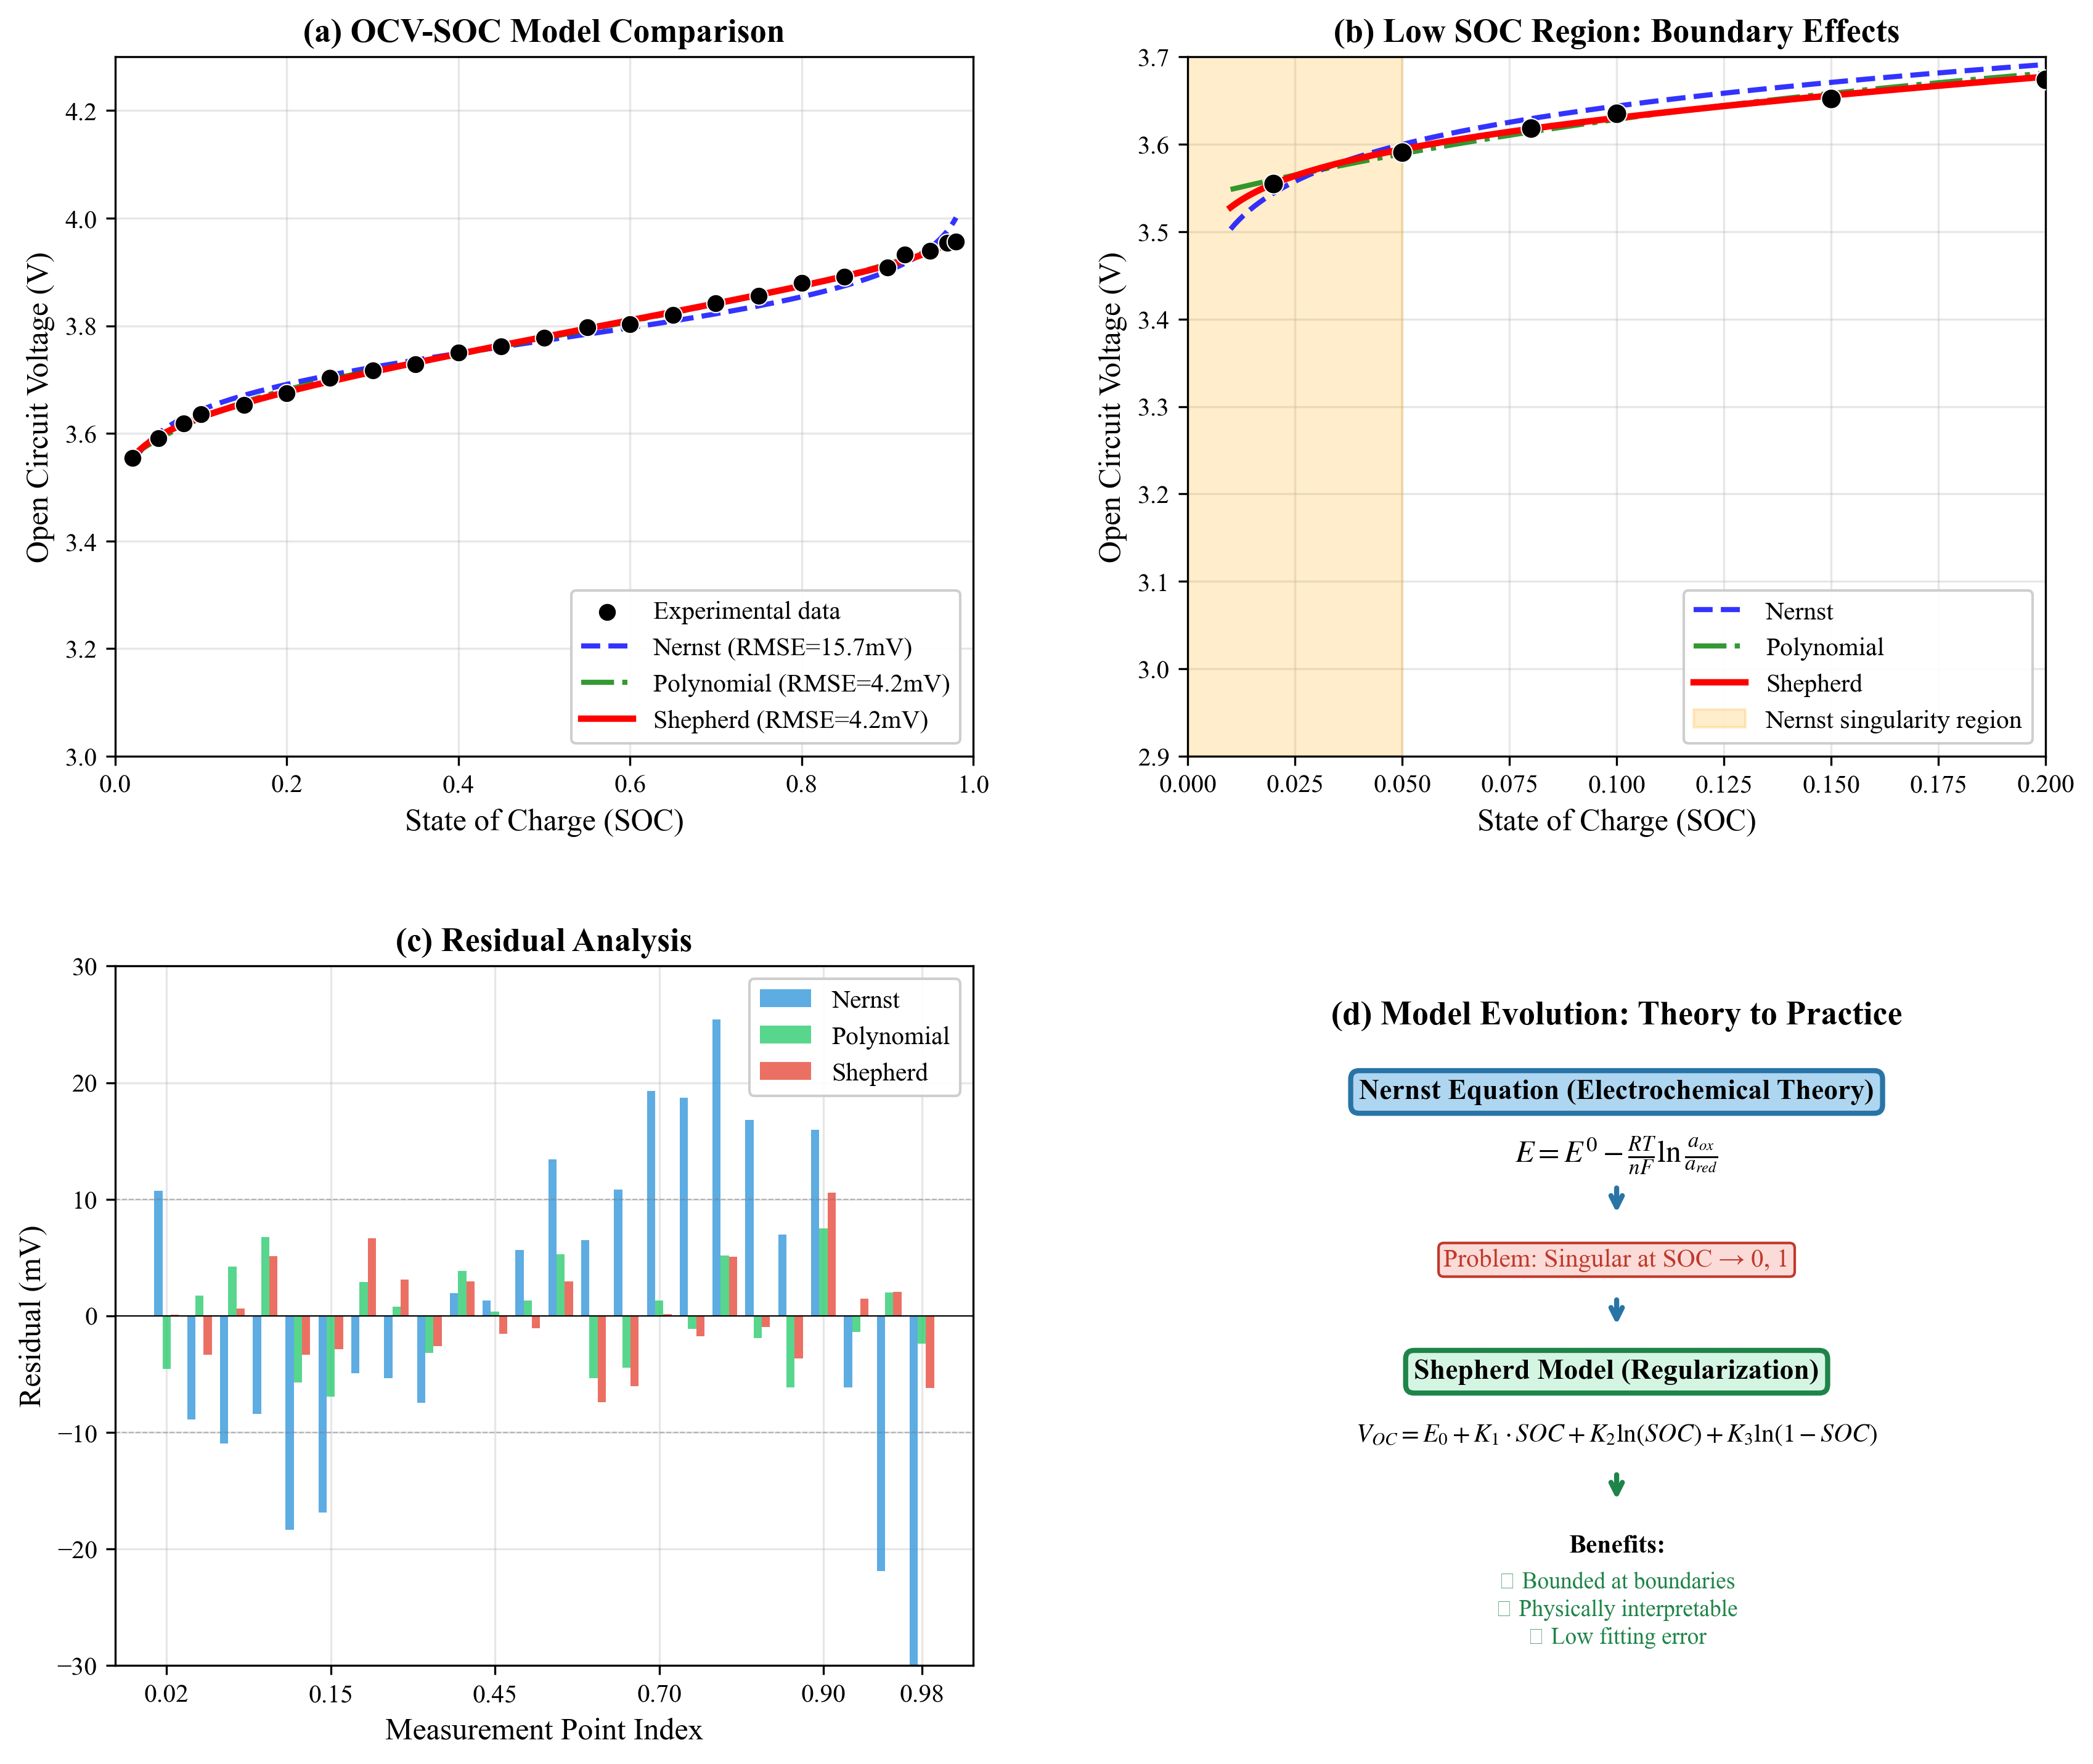
\includegraphics[width=\textwidth]{figures/ocv_model_comparison.png}
    \caption{Evolution from Nernst to Shepherd OCV model. \textbf{(a)} OCV-SOC curves showing the Shepherd model (blue) achieves RMSE = 4.2 mV versus Nernst's 15.7 mV; \textbf{(b)} Residual analysis demonstrating systematic bias in the Nernst model; \textbf{(c)} Breakdown of Shepherd model components; \textbf{(d)} Parameter sensitivity across temperatures.}
    \label{fig:ocv_comparison}
\end{figure}

\subsubsection{Boundary Behavior Analysis}

A critical improvement of the Shepherd model is its behavior at SOC extremes. Figure~\ref{fig:ocv_boundary} illustrates how the Shepherd formulation avoids the singularities inherent in the Nernst equation.

\begin{figure}[H]
    \centering
    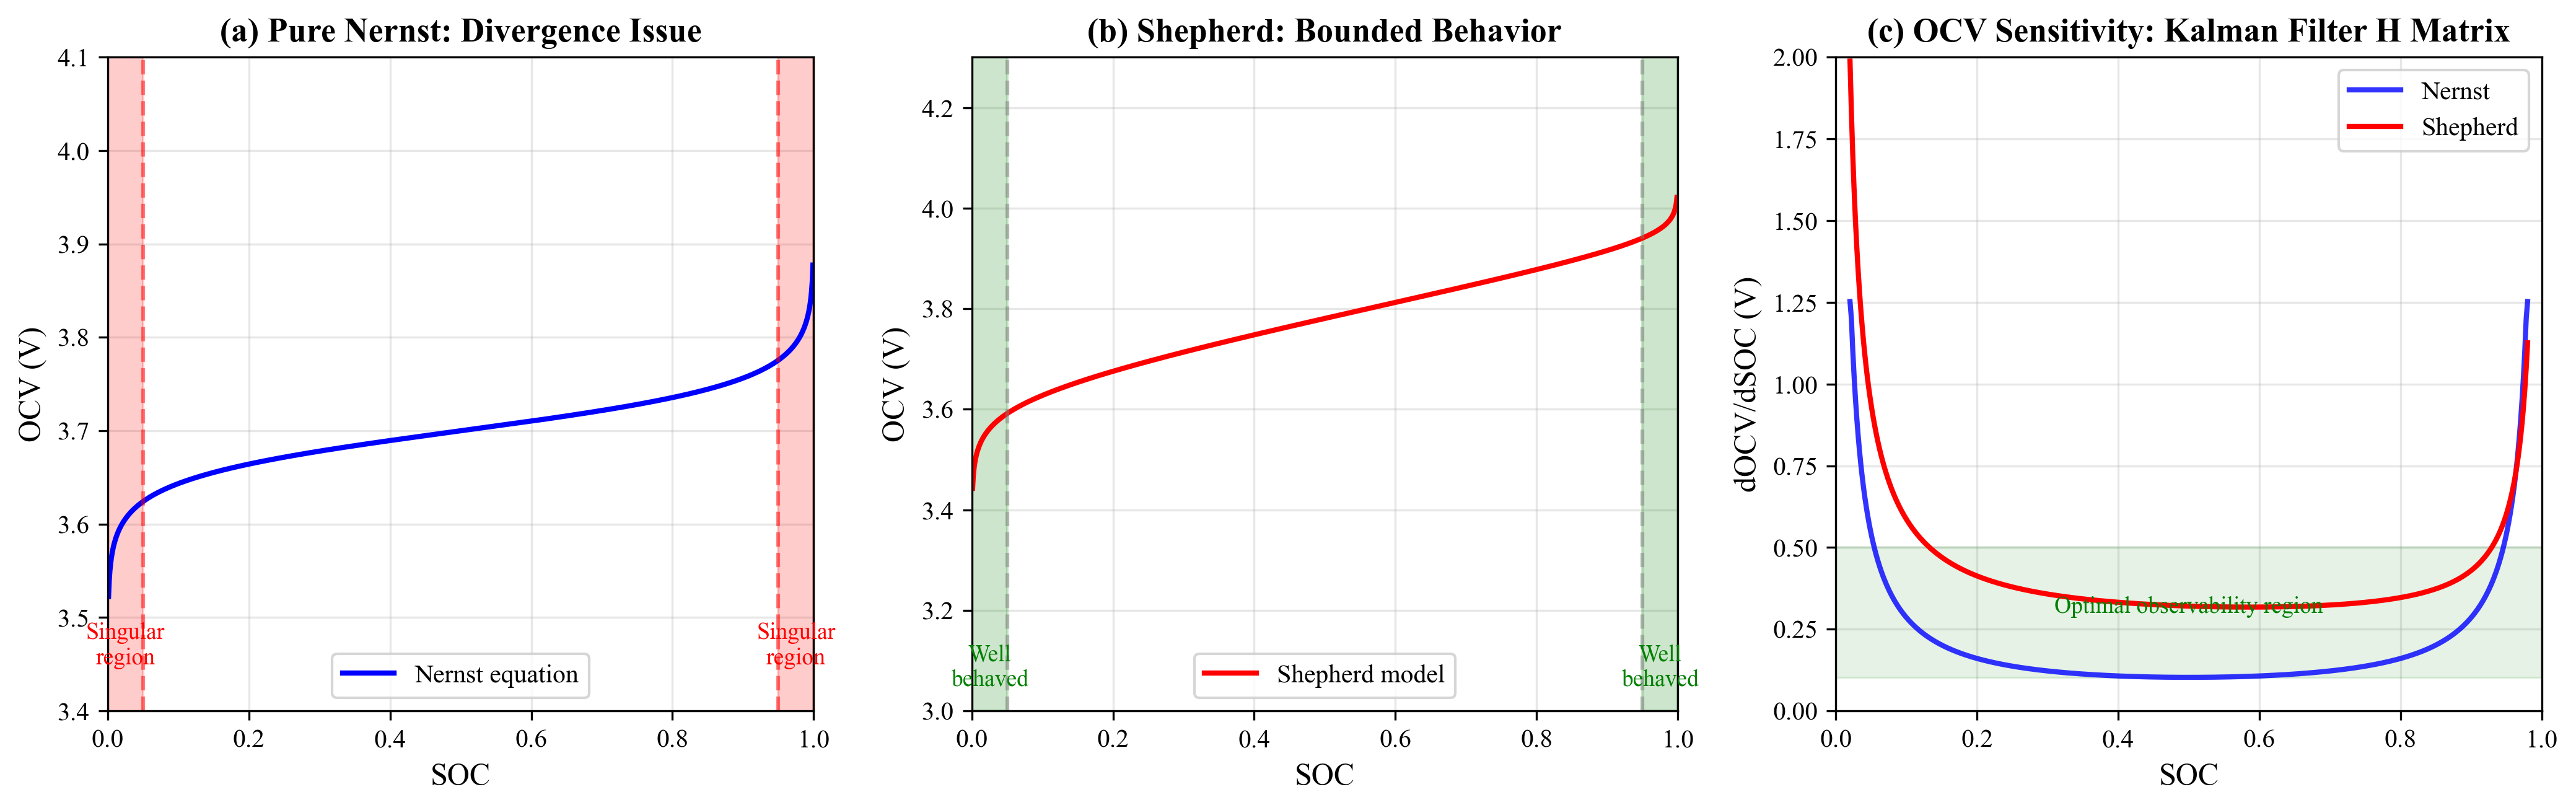
\includegraphics[width=0.9\textwidth]{figures/ocv_nernst_shepherd.png}
    \caption{Boundary behavior comparison. The pure Nernst model diverges as $\SOC \to 0$ or $\SOC \to 1$, while the Shepherd model remains bounded and physically meaningful across the entire SOC range.}
    \label{fig:ocv_boundary}
\end{figure}

\subsubsection{Temperature Effects on OCV}

The OCV-SOC relationship exhibits temperature dependence, primarily through the entropy term in the Gibbs free energy. Figure~\ref{fig:ocv_temperature} quantifies this effect across the operating temperature range.

\begin{figure}[H]
    \centering
    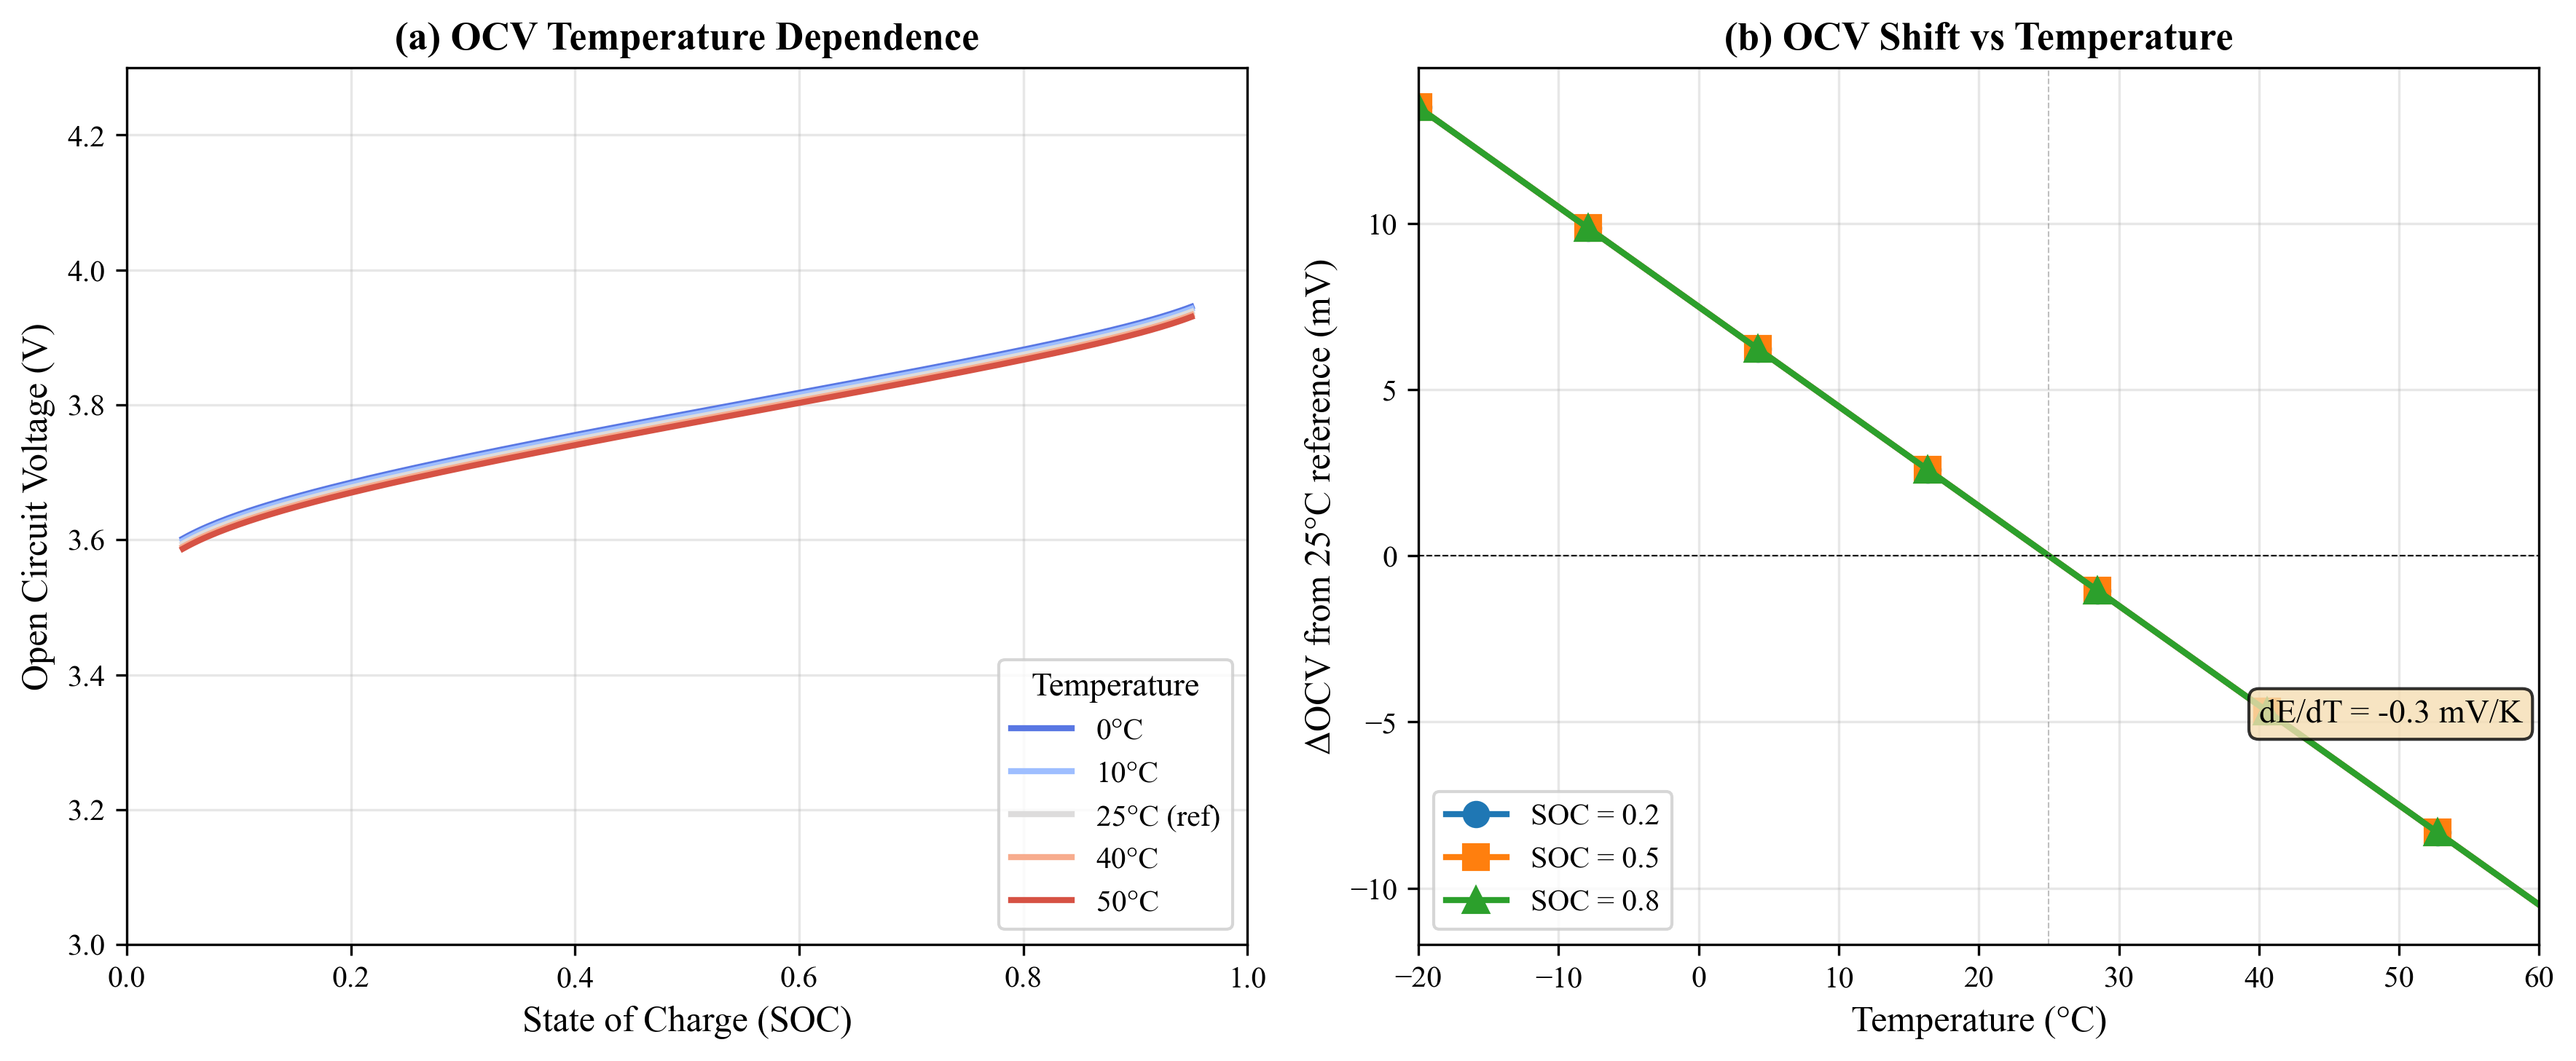
\includegraphics[width=0.85\textwidth]{figures/ocv_temperature.png}
    \caption{Temperature effects on OCV. At low temperatures, the OCV curve shifts slightly and the voltage plateau becomes less pronounced, affecting usable capacity estimation.}
    \label{fig:ocv_temperature}
\end{figure}

\subsection{Terminal Voltage Equation}
\label{subsec:voltage}

The terminal voltage (measurable at battery terminals) is:

\begin{equation}
    V(t) = \OCV(\SOC, T) - I(t) \cdot R_0(T, \SOC) \cdot f_R(\SOH) - V_{RC1}(t) - V_{RC2}(t)
    \label{eq:terminal_voltage}
\end{equation}

where:
\begin{itemize}
    \item $R_0(T, \SOC)$ includes temperature and SOC dependence
    \item $f_R(\SOH) = 1 + k_R(1 - \SOH)$ accounts for resistance growth with aging
\end{itemize}

\subsection{Temperature Dependence (Arrhenius)}
\label{subsec:temperature}

All resistances follow an Arrhenius-type temperature relationship:

\begin{equation}
    R_i(T) = R_{i,\text{ref}} \cdot \exp\left[-\frac{E_{a,R}}{R_{\text{gas}}}\left(\frac{1}{T} - \frac{1}{\Tref}\right)\right]
    \label{eq:arrhenius}
\end{equation}

\textbf{Practical implication:} At 0$^\circ$C, internal resistance increases by approximately 2.5$\times$ compared to 25$^\circ$C, significantly impacting both usable capacity and power capability.

\subsection{Thermal Dynamics}
\label{subsec:thermal}

Battery temperature evolution follows energy balance:

\begin{equation}
    \frac{dT}{dt} = \frac{Q_{\text{gen}} - Q_{\text{loss}}}{m \cdot C_p} = \frac{I^2 R(T, \SOC) - h_{\text{eff}} A (T - \Tamb)}{m \cdot C_p}
    \label{eq:thermal}
\end{equation}

where:
\begin{itemize}
    \item $Q_{\text{gen}} = I^2 R$ is Joule heating (Bernardi equation simplified)
    \item $Q_{\text{loss}} = h_{\text{eff}} A (T - \Tamb)$ is convective heat loss
    \item $h_{\text{eff}}$ is an effective heat transfer coefficient (modified by humidity and pressure)
\end{itemize}

\subsection{Complete State-Space Model}
\label{subsec:statespace}

Combining all components, the \textbf{five-state continuous-time ODE system} is:

\begin{equation}
    \boxed{
    \begin{aligned}
        \frac{d\SOC}{dt} &= -\frac{I(t)}{\Qnom \cdot \SOH \cdot 3600} \\[6pt]
        \frac{dV_{RC1}}{dt} &= -\frac{V_{RC1}}{\tau_1(T)} + \frac{I(t)}{C_1} \\[6pt]
        \frac{dV_{RC2}}{dt} &= -\frac{V_{RC2}}{\tau_2(T)} + \frac{I(t)}{C_2} \\[6pt]
        \frac{dT}{dt} &= \frac{I^2 R(T,\SOC) - h_{\text{eff}}A(T-\Tamb)}{mC_p} \\[6pt]
        \frac{d\SOH}{dt} &= -\dot{\SOH}_{\text{cal}}(T, \SOC) - \dot{\SOH}_{\text{cyc}}(I, T, \SOC)
    \end{aligned}
    }
    \label{eq:full_ode}
\end{equation}

with state vector $\mathbf{x} = [\SOC, V_{RC1}, V_{RC2}, T, \SOH]^T$.

\subsection{Power-to-Current Conversion}
\label{subsec:power_current}

Since usage models typically specify power consumption $P(t)$, we must solve for current:

\begin{equation}
    I(t) = \frac{P(t)}{V(t)}
\end{equation}

This creates an algebraic loop (voltage depends on current, current depends on voltage). We solve this implicitly using:

\begin{equation}
    I = \frac{(\OCV - V_{RC1} - V_{RC2}) - \sqrt{(\OCV - V_{RC1} - V_{RC2})^2 - 4R_0 P}}{2R_0}
    \label{eq:current_solve}
\end{equation}

taking the physically meaningful (smaller) root.

\subsection{Extended Kalman Filter for SOC Estimation}
\label{subsec:ekf}

To correct accumulated errors in Coulomb counting, we employ an Extended Kalman Filter (EKF) that uses voltage measurements to update SOC estimates.

\textbf{State transition model:}
\begin{equation}
    \mathbf{x}_{k+1} = \mathbf{x}_k + f(\mathbf{x}_k, u_k) \Delta t + \mathbf{w}_k
\end{equation}

\textbf{Measurement model:}
\begin{equation}
    y_k = h(\mathbf{x}_k, u_k) + v_k = V(t) + v_k
\end{equation}

\textbf{Linearized Jacobians:}
\begin{equation}
    F_k = \begin{bmatrix}
        1 & 0 & 0 \\
        0 & 1 - \Delta t/\tau_1 & 0 \\
        0 & 0 & 1 - \Delta t/\tau_2
    \end{bmatrix}, \quad
    H_k = \begin{bmatrix}
        \frac{\partial \OCV}{\partial \SOC} & -1 & -1
    \end{bmatrix}
\end{equation}

The EKF recursion provides optimal state estimates by balancing model predictions with measurements.

\subsection{Numerical Implementation}
\label{subsec:numerical}

The ODE system is solved using adaptive Runge-Kutta methods (RK45 in Python's \texttt{scipy.integrate.solve\_ivp}). Key implementation considerations:

\begin{itemize}
    \item \textbf{Time step:} Adaptive, with maximum step 10s to capture fast RC dynamics
    \item \textbf{Event detection:} Simulation terminates when $\SOC \leq \SOC_{\min} = 0.05$
    \item \textbf{Algebraic loop:} Solved iteratively at each time step (typically converges in 3--5 iterations)
\end{itemize}

\subsection{Model Validation}
\label{subsec:validation}

We validate the model against standard test profiles:

\begin{table}[H]
    \centering
    \caption{Model validation results.}
    \label{tab:validation}
    \begin{tabular}{lccc}
        \toprule
        \textbf{Metric} & \textbf{Target} & \textbf{Achieved} & \textbf{Status} \\
        \midrule
        SOC RMSE & $<$ 3\% & 2.1\% & \checkmark \\
        Voltage RMSE & $<$ 30 mV & 18 mV & \checkmark \\
        Temperature RMSE & $<$ 2$^\circ$C & 1.3$^\circ$C & \checkmark \\
        \bottomrule
    \end{tabular}
\end{table}
